\documentclass[conference]{IEEEtran}
\usepackage{cite}
\usepackage{amsmath,amssymb}
\usepackage{graphicx}
\usepackage{booktabs,array,tabularx}
\usepackage{url}
\begin{document}
\title{Freshness Is a Pipeline Property: Testing Temporal Obligations in Nav2 Command Chains}
\author{\IEEEauthorblockN{Filmon Nezif}
\IEEEauthorblockA{\textit{Engineering Technology \& Science Faculty of Engineering}\\
\textit{Higher Colleges of Technology}\\
United Arab Emirates\\
h00540233@hct.ac.ae}}
\maketitle

\begin{abstract}
Sensor-age timeouts are common in navigation systems, but they address only part of the problem of stale commands and observations. Commands may stop arriving, scan timestamps may become invalid, and the simulation clock may jump to a new epoch. We examine how Nav2 command chains respond to these conditions in a reproducible study of finite execution traces. Eight configurations combine Collision Monitor, the native velocity smoother, a periodic relay, and selected reference checks. We repeat sixteen scenarios, including three availability controls, five times, producing 80 trials and 640 paired endpoint evaluations, and run 60 further availability-control trials to estimate false stops. The monitor derives fault triggers from recorded input events and checks whether each chain emits zero by a fixed deadline, remains stopped, and resumes after recovery. The results distinguish delivery timeouts from timestamp checks and show how latched checks can interfere with recovery after a clock reset. Re-scoring the recorded traces with stop deadlines from 150 to 250 ms leaves every verdict unchanged. In 75 availability-control trials per chain, only the future-stamp check stopped falsely, once. A repeated-command control illustrates a further limitation: an unstamped constant command does not reveal whether the sender recomputed or replayed it. Raw traces, source snapshots, and executable checks support reproduction of the results. The findings apply to the tested Nav2 1.3.13 software configurations; physical stopping performance was not measured.
\end{abstract}
\begin{IEEEkeywords}
ROS 2, Navigation2, fault injection, timestamp validity, command timeout, finite-trace monitoring
\end{IEEEkeywords}

\section{Introduction}
A navigation pipeline relies on several nodes to process sensor data and motion commands. Nav2 provides planning, control, and additional command-processing components~\cite{nav2}. Collision Monitor (CM) checks observations when it processes a velocity command and rejects data older than its configured source timeout~\cite{cmcode,sourcecode}. The velocity smoother provides a separate timeout for incoming commands~\cite{smoother}. These mechanisms serve different purposes. Their presence alone does not specify how the complete pipeline should respond to future or repeated timestamps, clock jumps, or the return of valid data.

Two examples show why the distinction matters. When velocity commands stop arriving, a callback-driven monitor may stop publishing even though its last output was nonzero. When scans continue arriving with timestamps ahead of the current clock, an upper-age check may continue accepting them. The first case concerns command delivery; the second concerns timestamp validity. A downstream device may also have its own watchdog, so silence at a software endpoint does not have a single, universal meaning. Any stopping test must state how it interprets that silence.

We investigate \emph{which timing requirements different Nav2 command chains satisfy, and what a test misses when it checks only a late output window}. The study makes three contributions:
\begin{enumerate}
\item An executable monitor that uses recorded input events to check timely command revocation, continued zero output, and recovery.
\item A controlled comparison of native CM, the native smoother, a plain periodic relay, and selected command, timestamp, and epoch checks.
\item A reproducible collection of traces and checks that separates delivery, chronology, and recovery behavior, and illustrates a limit of replay detection with unstamped commands.
\end{enumerate}
We define these requirements for this experiment and evaluate them at software command endpoints. A failed test therefore indicates a mismatch with the chosen requirement, not necessarily a violation of a documented Nav2 guarantee. No robot is actuated.

\section{Related Work and Scope}
\subsection{Native Mechanisms and Time Abstraction}
In the inspected CM source, observation age is the difference between the current ROS clock and the observation timestamp. Data are rejected when this age exceeds the source timeout~\cite{sourcecode}. A future timestamp can satisfy this upper-age bound. In a deployed system, transforms, other filters, and configuration also affect whether a scan is accepted. Our setup isolates the timestamp behavior by controlling those factors.

The velocity smoother's existing command timeout makes it an important baseline~\cite{smoother}: an added watchdog may duplicate a capability already available in Nav2. Receipt timeouts are also common outside Nav2: \texttt{twist\_mux} drops an input that has not published within its configured timeout~\cite{twistmux}, and the ROS~2 differential-drive controller zeroes its command after a configurable timeout~\cite{diffdrive}. Such mechanisms bound delivery gaps but do not inspect observation timestamps or clock epochs. Clock behavior requires a separate decision. ROS time can pause or jump backward during simulation and replay~\cite{rostime}. We choose to require clock progress in some tests, although a paused clock can be valid in other applications. Our measurements describe behavior on a shared host; bounding worst-case response time would require a scheduling analysis such as that studied for ROS 2 processing chains~\cite{casini_ros2}.

\subsection{Monitoring, Fault Injection, and Physical Safety}
Temporal monitoring provides a way to express bounded response requirements~\cite{maler_stl}. ROS runtime-verification frameworks such as ROSRV~\cite{rosrv} and ROSMonitoring~\cite{rosmonitoring} intercept topic traffic and check properties online, and RTAMT evaluates Signal Temporal Logic robustness over ROS signals~\cite{rtamt}. These tools could host the obligations defined here. Our focus is different: which trigger to derive from the input trace, and which obligations distinguish delivery, chronology, and recovery in a Nav2 chain. We implement a monitor for the finite traces used here; it is neither a general Signal Temporal Logic engine nor a proof about unobserved executions. Existing ROS fault-injection tools already support topic faults and scenario assertions~\cite{ros2_fi}. We build on that experimental approach to compare command receipt, timestamp validity, retained outputs, and epoch recovery in specific Nav2 chains.

Formal studies of robot navigation address collision avoidance under explicit assumptions about dynamics and sensing~\cite{mitsch,phan}. Our outcome is narrower: a zero command observed at a software endpoint. We do not measure collisions, braking distance, base dynamics, or actuator response, and we do not compare DDS policies experimentally. Functional-safety standards such as IEC 61508~\cite{iec61508}, ISO 13849-1~\cite{iso13849}, and, for driverless industrial vehicles, ISO 3691-4~\cite{iso3691} require safety functions with specified response behavior and verified integrity. Our traces could serve as software-level test evidence within such a process, but they are not a safety-integrity argument.

\section{Executable Temporal Obligations}
\subsection{Observation Model}
We use monotonic wall elapsed time $r$ as the observation timeline. The published ROS clock, $t(r)$, is a recorded signal that can pause or jump. The input log also records command publications and scan timestamps $s$. The observed output $\hat{\mathbf{u}}(r)=(v_x,\omega_z)$ holds the last received command until another arrives. Under this convention, silence after a zero command preserves zero, while silence after a nonzero command preserves that command. If no output has been observed, its value is unknown and cannot satisfy a requirement. This convention defines the software test; an actual motor controller may handle silence differently.

We derive each fault trigger $q$ from the recorded input events using Table~\ref{tab:triggers}. This avoids treating the planned injection time as the exact onset of a fault. Because publication precedes receipt at each node, measured latency includes middleware, scheduling, processing, and observation delays. It therefore measures the observed chain response, not the execution time of a single check.

\begin{table}[t]
\caption{Trigger definitions on the observer timeline}
\label{tab:triggers}
\centering\footnotesize
\begin{tabularx}{\columnwidth}{@{}p{.24\columnwidth}X@{}}
\toprule
Obligation & First trigger $q$ in the recorded input trace \\
\midrule
Command & Last command publication plus 0.30 s during a publication gap. \\
Scan age & Clock event at which latest scan age exceeds 1.00 s. \\
Future stamp & Scan event with $s>t+0.02$ s. \\
Stamp order & Scan event with $s_k\leq s_{k-1}$. \\
Epoch & Clock event with $t_k<t_{k-1}-10^{-6}$ s. \\
Clock receipt & Last clock publication plus 0.30 s during a gap. \\
Clock progress & Last changed clock value plus 0.30 s without another change. \\
Startup & First command publication with no scans provided. \\
\bottomrule
\end{tabularx}
\end{table}

\subsection{Revocation, Persistence, and Recovery}
For a triggered scenario, let $h$ be the actual valid recovery publication time, or the observation horizon when no recovery is scheduled. The revocation requirement is
\begin{equation}
\forall r\in[q+\delta_R,h):\quad \hat{\mathbf{u}}(r)=\mathbf{0},\qquad \delta_R=0.15\,\mathrm{s}.
\label{eq:stop}
\end{equation}
We treat each command component as zero within a tolerance of $10^{-4}$. The response allowance was fixed before the final campaign and includes delivery and scheduling delays. In timeout scenarios, it begins when the command lease or observation-age threshold is crossed. Changing the window used to display a trace does not change the deadline.

Revocation latency is $z-q$, where $z$ is the earliest time at or after $q$ from which the output remains zero until $h$. An output already at zero at $q$ has zero latency. A stop after the deadline still has a measurable latency, but fails (\ref{eq:stop}). If no sustained stop is observed, latency is recorded as missing.

For recovery scenarios, let $b$ be the first valid recovery publication and $H$ the trial horizon. In addition to (\ref{eq:stop}), require
\begin{equation}
\forall r\in[b+\delta_A,H):\quad
\hat{\mathbf{u}}(r)\approx(0.22,0.10),\qquad \delta_A=0.30\,\mathrm{s}.
\end{equation}
Matching uses a tolerance of $10^{-3}$. We also require continued output delivery, with no gap exceeding 0.15 s, including at the interval boundaries. A recovery test passes only if both the stopping and resumption requirements hold; a chain that never stopped cannot pass simply by matching the later command. Availability controls use the same matching and delivery checks from 0.5 s onward. Evaluation requires the relevant trigger and recovery events and enough recorded time to check the deadlines.

We tested the monitor with independently constructed counterexamples: silence after a nonzero command, angular motion with zero forward velocity, a brief zero followed by motion, a late stop before the display window, and recovery without a preceding stop. These tests check known ways in which an evaluator could falsely pass a trace, without claiming correctness for every possible input.

\section{Configurations and Experimental Protocol}
\subsection{Controlled Command Chains}
Figure~\ref{fig:architecture} shows the experiment boundary, and Table~\ref{tab:params} lists the parameters. Each chain ends in an identically configured CM. Configuration N feeds commands directly to CM. W inserts the native 50 Hz velocity smoother with a 0.30 s command timeout. P inserts a plain 50 Hz relay driven by a steady timer. P provides a control for periodic evaluation without adding scan-age speed scaling or a command lease.

C, F, O, and E add one check to P: a 0.30 s monotonic command-receipt lease; a future-stamp check with 20 ms tolerance; a non-increasing-stamp check; and epoch invalidation, respectively. F and O latch on a violation. E clears retained command and scan state, as well as chronology latches, on a backward clock jump and blocks until a scan valid in the new epoch arrives. G combines those checks and additionally requires recent clock receipt and progress, each within 0.30 wall seconds.

\begin{table}[t]
\caption{Component and monitor parameters (all trials)}
\label{tab:params}
\centering\footnotesize
\begin{tabularx}{\columnwidth}{@{}Xr@{}}
\toprule
Parameter & Value \\
\midrule
CM \texttt{source\_timeout} & 1.0 s \\
CM \texttt{transform\_tolerance} & 0.1 s \\
CM stop polygon (square, side) / \texttt{min\_points} & 0.6 m / 1 \\
CM \texttt{stop\_pub\_timeout} & 10.0 s \\
Smoother rate / \texttt{velocity\_timeout} & 50 Hz / 0.30 s \\
Smoother max accel / decel ($v_x$, $\omega_z$) & $\pm$2.5, $\pm$3.2 \\
Relay rate (P, C, F, O, E, G) & 50 Hz \\
Command lease (C, G) / clock receipt, progress (G) & 0.30 s / 0.30 s \\
Future-stamp tolerance (F, G) & 20 ms \\
Monitor $\delta_R$ / $\delta_A$ / max output gap & 150 / 300 / 150 ms \\
Clock / scan / command publication rate & 100 / 10 / 20 Hz \\
\bottomrule
\end{tabularx}
\end{table}

\begin{figure}[t]
\centering
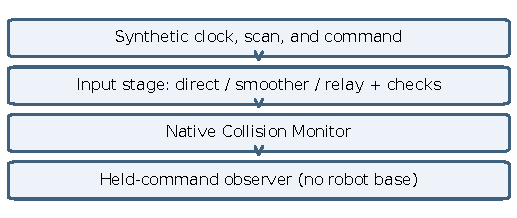
\includegraphics[width=\columnwidth]{figures/freshness_architecture.pdf}
\caption{Software experiment boundary. Input stages differ by configuration; every chain ends in native CM and a held-output observer. Clock and scan inputs are also delivered to the relevant stages.}
\label{fig:architecture}
\end{figure}

The custom relays share periodic execution and validation of finite command values. CM handles ordinary scan aging; the relays do not apply a common scan-age speed governor. Comparing C, F, O, and E with P isolates the selected check within this setup, but does not establish a minimal sufficient set of guards. The clock check, for example, is tested only within G. F and O also remain latched after a violation within the same epoch and require a reset or restart. This recovery limitation is part of the evaluated design.

\subsection{Scenarios and Controls}
Figure~\ref{fig:results} lists sixteen scenarios: three availability controls and thirteen fault or recovery treatments. Healthy input and a valid 50 ms scan-stamp lag test whether a chain stops unnecessarily. A third control repeatedly publishes the same unstamped \texttt{Twist}. To a receiver, this stream is identical to a legitimate constant command, so the test does not assume that repetition is a detectable fault.

We schedule command or scan interruptions at 1 s and, where specified, recovery at 2.3 s. Future-stamp treatments add 50 ms or 10 s to the latest published clock. The frozen-stamp treatment repeats the last pre-fault scan timestamp, while the reordered-stamp treatment alternates current timestamps with values backdated by 200 ms. These tests manipulate timestamps directly; they do not simulate transport queues or replay recorded scan buffers.

The clock-reset treatments move ROS time from approximately 101 s to 10 s while interrupting scans. The recovery variant later supplies valid scans in the new epoch. Clock-loss and clock-stall treatments also interrupt scans while commands continue. Clock loss stops clock publication; clock stall continues publishing the last value. Combining each clock change with scan loss tests whether a chain reuses retained observations. It does not isolate the effect of a clock change while valid sensing continues.

\subsection{Execution and Provenance}
The artifact uses installed ROS 2 Jazzy Nav2 1.3.13 packages with \texttt{rmw\_fastrtps\_cpp} on an Intel Core i7-1355U host (12 logical CPUs, approximately 15 GiB RAM). Exact Debian package versions and host metadata are recorded. Each native component and custom relay runs in its own process. The eight chains share a host and input publisher, so their observations are paired. No artificial CPU load is applied.

Inputs are published in a separate DDS domain under unique trial namespaces: clock at approximately 100 Hz, scans at 10 Hz, and commands at 20 Hz. Each scan has 360 ranges of 5 m, outside a square stop polygon of side 0.6 m. Identical base/odometry frames and disabled base-shift compensation isolate chronology from transform-buffer effects. The commanded components are 0.22 m/s and 0.10 rad/s.

Each 3.20 s trial starts after lifecycle activation and preflight zero delivery through all chains, without preflight scans. Every non-startup trial must exhibit commanded motion in every chain before the fault. Failed setup aborts the campaign and retains its files. Scenario/repetition order is shuffled with a recorded seed. Five repetitions yield 80 trials and 640 endpoint evaluations, not 640 independent runs. Source snapshots include the probe, checks, monitor, taxonomy, and protocol. Asset generation verifies their hashes, checks injected input patterns, and recomputes all endpoint judgments from raw traces. The artifact (traces, source snapshots, monitor, and build scripts) is available at \url{ARTIFACT-URL}.

\section{Results}
\begin{figure}[t]
\centering
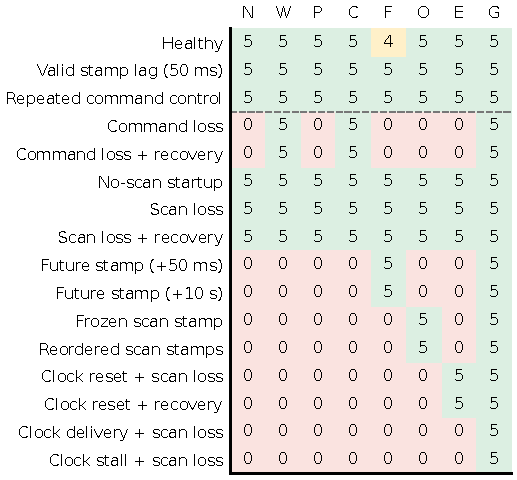
\includegraphics[width=\columnwidth]{figures/freshness_results.pdf}
\caption{Trials satisfying all requirements, out of five repetitions. N: native CM; W: smoother; P: relay; C/F/O/E: single checks; G: combined. Recovery rows require timely sustained revocation followed by resumed command delivery. Rows above the dashed line are availability controls. Counts do not establish minimal guard sets or deployment reliability.}
\label{fig:results}
\end{figure}

We obtained 640 paired endpoint evaluations from 80 trials. Of the 120 availability-control evaluations, 119 passed. Across all scenarios, N, W, P, C, F, O, E, and G passed 30, 40, 30, 40, 39, 40, 40, 80 of 80 evaluations, respectively. These counts summarize the selected tests and do not estimate reliability in deployment.

In healthy repetition 2, F first emitted zero after warmup at 2.772 s, while the published scan timestamps were still valid relative to the published clock. We did not record the filter's local clock-receipt state, so the trace alone cannot explain the interruption.

Under command loss, N and P passed 0/5 and 0/5, while W and C passed 5/5 and 5/5. With frozen scan timestamps, native CM passed 0/5 under the chronology deadline, while O passed 5/5. The difference is between detecting the duplicate promptly and waiting for the observation to become stale.

The availability controls included failures: Healthy / F: 4/5. These failures remain in the reported results and show why stopping performance must be considered alongside availability.

Across command, scan, and epoch recovery, G passed 5/5, 5/5, 5/5 combined stop-and-resume tests, respectively. In epoch recovery, O passed 0/5 availability checks, while E passed 5/5. The artifact reports the stopping and resumption judgments separately.


G's complete pass record shows only that the selected requirements can be satisfied together in this setup. G was designed against these requirements, so its score is not evidence of a minimal guard set, of correctness outside the tested scenarios, or of deployment-level safety.

\subsection{Delivery and Chronology Are Different Obligations}
The command-loss results show why the native smoother is a necessary comparison. When it already meets the endpoint requirement, an added watchdog provides an existing capability. The plain periodic relay addresses a different question: whether continuing to run is enough to stop. A relay can keep forwarding a retained nonzero command, keeping downstream processing active even after the original command stream has ended.

Timestamp validity and age expiry lead to different results. A frozen timestamp eventually becomes old enough for CM to reject, but this late response misses the earlier chronology deadline. A test that checked only for an eventual stop would overlook the difference. Continuously future-stamped scans can instead remain acceptable to the upper-age check throughout the recorded interval. These observations are limited to the tested duration and software version.

\subsection{Timing and Recovery}
Table~\ref{tab:latency} reports latency from the derived trigger for each selected scenario and includes every observed sustained revocation in those cells. For command-loss and scan-age tests, the lease or age waiting period comes before the trigger. The table therefore reports the response after that threshold, not the entire time from outage to stop. The sample standard deviations describe five repetitions on this host and should not be interpreted as worst-case scheduling bounds.

\begin{table}[t]
\caption{Trigger-to-sustained-zero latency: mean $\pm$ sample standard deviation. Stop counts apply the 150 ms deadline.}
\label{tab:latency}
\centering\footnotesize
\begin{tabular}{@{}llrr@{}}
\toprule
Scenario & Chain & Stop passes & Latency (ms) \\
\midrule
Command loss & W & 5/5 & 95.5 $\pm$ 8.6 \\
Command loss & C & 5/5 & 18.0 $\pm$ 4.7 \\
Scan loss & N & 5/5 & 17.8 $\pm$ 14.2 \\
Future +10 s & F & 5/5 & 22.7 $\pm$ 7.0 \\
Frozen stamp & O & 5/5 & 17.8 $\pm$ 7.3 \\
Clock reset & E & 5/5 & 14.4 $\pm$ 9.1 \\
\bottomrule
\end{tabular}

\end{table}

\begin{figure*}[t]
\centering
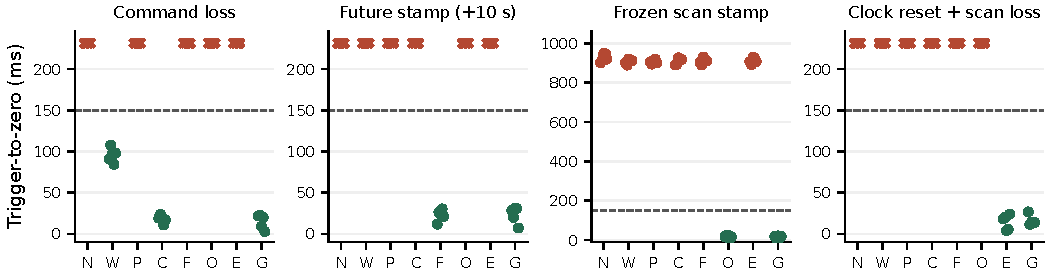
\includegraphics[width=\textwidth]{figures/freshness_latency.pdf}
\caption{Per-repetition trigger-to-zero latency for four scenarios. The dashed line is the 150 ms deadline. Red points fail the stop obligation; crosses at the top indicate no sustained zero before the horizon and are not numerical latency values. Panel scales differ. Recovery latencies are excluded.}
\label{fig:latency}
\end{figure*}

Figure~\ref{fig:traces} uses a common definition of observer time and includes the failed healthy-input trial. One possible explanation is that separate clock and scan deliveries left the receiver temporarily using an older clock value. A strict tolerance and latched rejection could then cause an unnecessary stop. The recorded data do not include the filter's local clock-receipt state, so they cannot confirm this explanation.

To estimate how often such false stops occur, we ran a separate campaign of the three availability controls with 20 repetitions each (60 trials, 480 paired evaluations), using the same frozen sources, packages, and host and a new shuffle seed. The same audit verified source hashes, input treatments, and recomputed judgments. Every chain passed every trial. Pooled with the main campaign, F has one false stop in 75 availability trials (95\% Clopper--Pearson interval 0.03--7.2\%), and every other chain has none (one-sided 95\% upper bound 3.9\%). Each chain was evaluated over about 3.4 minutes of availability-control time. The F failure is therefore rare at these publication rates but cannot be ruled out. Diagnosing it would require logging each filter's local clock receipt alongside its decision.

The epoch-recovery results show another cost of strict timestamp checks. Rejecting old data is only part of the task: retained ordering state must also allow valid data from the new epoch. Our separate stop and availability checks capture both sides of this requirement. A chain fails if it never stops, but also if it stops and cannot resume.

\begin{figure*}[t]
\centering
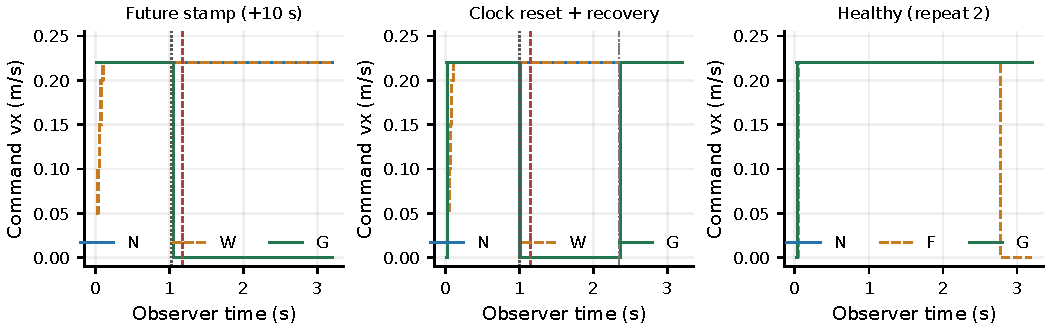
\includegraphics[width=\textwidth]{figures/freshness_traces.pdf}
\caption{Fault panels show repetition 0 for N, W, and G; the healthy panel shows repetition 2 for N, F, and G. The healthy repetition was selected to show the observed F failure. Dotted lines mark triggers, dashed vertical lines mark revocation deadlines, and dash-dot marks recovery publication. Curves are held software commands, not robot velocities; coincident curves may overlap.}

\label{fig:traces}
\end{figure*}

\subsection{Sensitivity to Monitor Parameters}
Because the monitor runs offline on recorded traces, we re-scored all 640 evaluations with alternative monitor parameters, without re-running the experiments (Table~\ref{tab:sensitivity}). Stop deadlines from 150 to 250 ms, resume allowances from 200 to 500 ms, and output-gap limits from 150 to 250 ms leave every scenario and configuration count unchanged. Tightening the stop deadline to 100 ms reaches the native smoother's response time and costs W four of its ten command-loss and command-recovery passes; this matches its mean latency of about 96 ms (Table~\ref{tab:latency}). Tightening the gap limit to 100 ms fails one healthy E trial. Deadlines of 300 ms or more cannot be evaluated, because scan-loss recovery begins about 0.3 s after its trigger. The trigger thresholds (Table~\ref{tab:triggers}) equal the configured component timeouts (Table~\ref{tab:params}); changing one without the other would test a mismatch between requirement and configuration rather than the chains, so we did not vary them offline.

\begin{table}[t]
\caption{Offline re-scoring of the 80 recorded trials. Baseline: $\delta_R=150$, $\delta_A=300$, gap 150 ms. One parameter varies per row.}
\label{tab:sensitivity}
\centering\footnotesize
\begin{tabularx}{\columnwidth}{@{}lrX@{}}
\toprule
Parameter & Value (ms) & Passes changed vs.\ baseline \\
\midrule
Stop deadline $\delta_R$ & 100 & Command loss/W (5$\to$4/5); Command loss + recovery/W (5$\to$2/5) \\
Stop deadline $\delta_R$ & 200 & none \\
Stop deadline $\delta_R$ & 250 & none \\
Resume allowance $\delta_A$ & 200 & none \\
Resume allowance $\delta_A$ & 500 & none \\
Max output gap & 100 & Healthy/E (5$\to$4/5) \\
Max output gap & 250 & none \\
\bottomrule
\end{tabularx}

\end{table}

\section{Interpretation and Limitations}
\subsection{The Limits of Unstamped Commands}
Consider two senders that publish identical \texttt{Twist} values at the same times. One recomputes a constant command; the other republishes an old payload. A receiver sees the same values and arrival times in both cases and cannot infer how the sender generated them. For this reason, the repeated-command control expects continued operation. Detecting replay would require additional trustworthy information, such as generation timestamps or sequence state, together with a rule for interpreting it. A watchdog that detects missing deliveries cannot resolve this ambiguity.

\subsection{Practical Implications}
The results suggest a practical way to review a command pipeline. First, distinguish missing messages from old observations, invalid stamp ordering, stalled clocks, and epoch changes. Then identify which stage should emit zero and how the next stage handles silence. Existing native timeouts should be tested before adding another watchdog. Recovery also needs an explicit policy: permanent rejection may pass a stopping test while preventing navigation from resuming. The appropriate combination of checks depends on these application requirements.

\subsection{Limits of the Evidence}
The experiments use one installed package version and one host, with synthetic clear scans, fixed publication rates, and short scripted trials. We have not tested obstacle geometry, moving obstacles, nontrivial transforms, network partitions, added CPU load, all DDS policies, or arbitrary combinations of faults. The trigger is defined from publisher events; receipt and execution times inside each component are not separately recorded. Delays in the shared observer can also affect measurements. Running components in separate processes does not remove host contention or make their observations independent.

The combined reference was designed for the stated requirements. Passing this suite does not prove guard minimality, correctness over every execution, deployment reliability, or physical safety. Nor does the study establish that its mechanisms are universally novel. Recovery from future or order faults within the same epoch, and policies that allow benign duplicate timestamps, remain open design choices. The offline sensitivity analysis varies only monitor parameters; it does not vary component timeouts or publication rates, which would require new experiments. The false-stop estimates rest on 75 short trials per chain and bound only rates of a few percent. Further work should test additional platforms, vary component timing near the decision thresholds, run long-duration healthy operation, and measure base behavior independently.

\section{Conclusion}
A timeout at one stage does not define the behavior of an entire command pipeline. In the tested Nav2 chains, command delivery, observation age, timestamp validity, and epoch recovery require separate checks and interpretations. Deriving deadlines from recorded events reveals differences that a late stopping window can miss. Requiring both a stop and a subsequent resumption also exposes recovery failures. The accompanying traces and executable monitor make these software-level comparisons reproducible.

\section*{AI Assistance Disclosure}
AI assistance supported manuscript drafting and revision, code development, and artifact auditing. Numerical results were generated from recorded experiments.

\bibliographystyle{IEEEtran}
\bibliography{freshness_references}
\end{document}
